\documentclass[11pt]{article}

\usepackage[a4paper,margin=0.75in]{geometry}
\usepackage{amsmath,amssymb}
\usepackage{graphicx}
\usepackage{booktabs}
\usepackage{array}
\usepackage{float}
\usepackage{hyperref}
\usepackage{enumitem}
\usepackage{xcolor}
\usepackage{tikz}
\usetikzlibrary{positioning,arrows.meta,shapes.geometric}

\setlist{nosep}
\renewcommand{\arraystretch}{1.3}

\tikzset{
layer/.style={
draw,
rounded corners,
minimum width=2.2cm,
minimum height=0.9cm,
align=center,
fill=blue!10
},
arrow/.style={
-{Latex[length=3mm]},
thick
}
}

\begin{document}

%%%%%%%%%%%%%%%%%%%%%%%%%%%%%%%%%%%%%%%%%%%%%%%%%%%%%%%%%%%%

\begin{center}

{\Large\textbf{Shiv Nadar University Chennai}}

\vspace{3mm}

{\large\textbf{CS3807 -- Deep Learning Laboratory}}

\vspace{3mm}

{\Large\textbf{Experiment 4}}

\vspace{2mm}

{\Large\textbf{Comparative Study of Deep Convolutional Neural}}

{\Large\textbf{Network Architectures Using Transfer Learning}}

\end{center}

\vspace{5mm}

\begin{tabular}{|p{4cm}|p{8cm}|p{2cm}|}
\hline
Degree \& Branch &
B.Tech Artificial Intelligence \& Data Science &
Semester V\\
\hline
Subject Code \& Name &
CS3807 -- Deep Learning Laboratory &
AY: 2026--27\\
\hline
\end{tabular}

%%%%%%%%%%%%%%%%%%%%%%%%%%%%%%%%%%%%%%%%%%%%%%%%%%%%%%%%%%%%

\section*{1. Objective}

The objectives of this experiment are

\begin{itemize}

\item Study the evolution of deep CNN architectures.

\item Compare LeNet-5, AlexNet, VGG16, GoogleNet and ResNet.

\item Understand transfer learning.

\item Fine tune pretrained CNN models.

\item Compare classification performance of different architectures.

\end{itemize}

%%%%%%%%%%%%%%%%%%%%%%%%%%%%%%%%%%%%%%%%%%%%%%%%%%%%%%%%%%%%

\section*{2. Learning Outcomes}

After completing this experiment students will be able to

\begin{enumerate}

\item Explain modern CNN architectures.

\item Differentiate LeNet, AlexNet, VGG16, GoogleNet and ResNet.

\item Implement transfer learning.

\item Fine tune pretrained CNN models.

\item Compare CNN architectures using performance metrics.

\end{enumerate}

%%%%%%%%%%%%%%%%%%%%%%%%%%%%%%%%%%%%%%%%%%%%%%%%%%%%%%%%%%%%

\section*{3. Introduction}

Deep Convolutional Neural Networks have become the dominant models for
computer vision applications because they automatically learn hierarchical
features from images. The evolution of CNNs has focused on improving
classification accuracy while reducing computational complexity and
training difficulties.

The progression of CNN architectures began with LeNet-5 and has evolved
through AlexNet, VGGNet, GoogleNet, and ResNet. Each architecture
introduced important innovations that significantly improved image
classification performance.

%%%%%%%%%%%%%%%%%%%%%%%%%%%%%%%%%%%%%%%%%%%%%%%%%%%%%%%%%%%%

\section*{4. Evolution of CNN Architectures}

\begin{center}

\begin{tabular}{|c|c|p{7cm}|}

\hline

Model & Year & Major Contribution\\

\hline

LeNet-5 & 1998 &
First practical convolutional neural network\\

\hline

AlexNet & 2012 &
ReLU activation, Dropout and GPU training\\

\hline

VGG16 & 2014 &
Uniform $3\times3$ convolution filters\\

\hline

GoogleNet & 2014 &
Inception modules for multi-scale feature extraction\\

\hline

ResNet & 2015 &
Residual learning using skip connections\\

\hline

\end{tabular}

\end{center}

%%%%%%%%%%%%%%%%%%%%%%%%%%%%%%%%%%%%%%%%%%%%%%%%%%%%%%%%%%%%

\section*{5. LeNet-5}

LeNet-5 was proposed by Yann LeCun in 1998 for handwritten digit
recognition. It consists of two convolution layers, two average pooling
layers and fully connected layers. It demonstrated that convolutional
networks could automatically learn image features without handcrafted
feature extraction.

Advantages

\begin{itemize}

\item Small number of parameters

\item Fast training

\item Suitable for OCR

\end{itemize}

%%%%%%%%%%%%%%%%%%%%%%%%%%%%%%%%%%%%%%%%%%%%%%%%%%%%%%%%%%%%

\section*{6. AlexNet}

AlexNet won the ImageNet Challenge in 2012 by reducing the
classification error significantly. It introduced ReLU activation,
Dropout regularization and GPU training.

Major innovations

\begin{itemize}

\item ReLU activation

\item Dropout

\item GPU implementation

\item Data augmentation

\end{itemize}

%%%%%%%%%%%%%%%%%%%%%%%%%%%%%%%%%%%%%%%%%%%%%%%%%%%%%%%%%%%%

\section*{7. VGG16}

VGG16 demonstrated that using multiple small $3\times3$ convolution
filters could outperform larger filters while increasing network depth.

Advantages

\begin{itemize}

\item Excellent feature extraction

\item Simple architecture

\item High classification accuracy

\end{itemize}

%%%%%%%%%%%%%%%%%%%%%%%%%%%%%%%%%%%%%%%%%%%%%%%%%%%%%%%%%%%%

\section*{8. Comparison of Architectures}

\begin{center}

\begin{tabular}{|l|c|c|c|}

\hline

Architecture &
Depth &
Parameters &
Main Contribution\\

\hline

LeNet-5 &
7 &
60K &
First CNN\\

AlexNet &
8 &
61M &
ReLU + Dropout\\

VGG16 &
16 &
138M &
Deep 3$\times$3 filters\\

GoogleNet &
22 &
6.8M &
Inception Modules\\

ResNet50 &
50 &
25.6M &
Residual Learning\\

\hline

\end{tabular}

\end{center}

%%%%%%%%%%%%%%%%%%%%%%%%%%%%%%%%%%%%%%%%%%%%%%%%%%%%%%%%%%%%
\section*{9. GoogleNet (Inception Network)}

GoogleNet, proposed by Szegedy \textit{et al.} in 2014, introduced the
\textbf{Inception Module}, which performs multiple convolution operations
in parallel using different filter sizes. Instead of using only a single
kernel size, GoogleNet simultaneously applies $1\times1$, $3\times3$,
$5\times5$ convolutions and max pooling. The outputs are concatenated to
obtain multi-scale feature representations.

The use of $1\times1$ convolutions before larger kernels reduces the
number of trainable parameters and computational complexity.

Advantages

\begin{itemize}
\item Multi-scale feature extraction.
\item Fewer parameters than VGG16.
\item High computational efficiency.
\item Better classification performance.
\end{itemize}

%%%%%%%%%%%%%%%%%%%%%%%%%%%%%%%%%%%%%%%%%%%%%%%%%%%%%%%%%%%%

\section*{10. ResNet}

Increasing CNN depth often causes the \textbf{vanishing gradient problem},
making optimization difficult. ResNet solves this issue using
\textbf{skip (residual) connections}, allowing gradients to flow directly
through the network.

Instead of learning $H(x)$, ResNet learns $F(x)=H(x)-x$, thus
$\text{Output} = F(x)+x$, where $F(x)$ is the residual mapping and
$x$ is the identity mapping.

\begin{figure}[H]
\centering

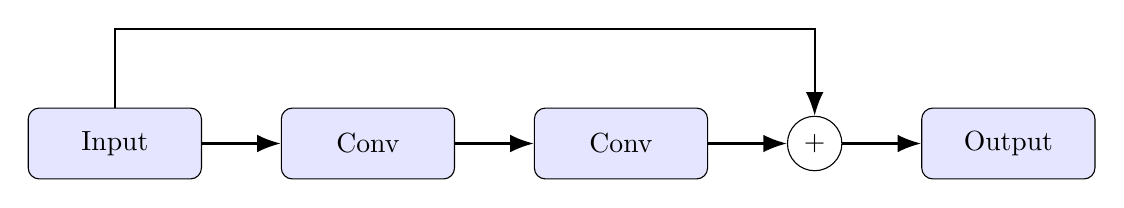
\begin{tikzpicture}[node distance=1cm]

\node[layer](input){Input};
\node[layer,right=of input](conv1){Conv};
\node[layer,right=of conv1](conv2){Conv};
\node[circle,draw,right=of conv2](add){+};
\node[layer,right=of add](output){Output};

\draw[arrow](input)--(conv1);
\draw[arrow](conv1)--(conv2);
\draw[arrow](conv2)--(add);
\draw[arrow](add)--(output);

\draw[arrow]
(input)
|-([yshift=10mm]conv2.north)
-| (add.north);

\end{tikzpicture}

\caption{Residual Block in ResNet}
\end{figure}

Advantages

\begin{itemize}
\item Eliminates vanishing gradients.
\item Enables very deep neural networks.
\item Faster convergence.
\item High ImageNet accuracy.
\end{itemize}

%%%%%%%%%%%%%%%%%%%%%%%%%%%%%%%%%%%%%%%%%%%%%%%%%%%%%%%%%%%%

\section*{11. Dilated Convolution}

Dilated convolution (also called atrous convolution) increases the
receptive field without increasing the number of parameters.
The dilation rate $D$ determines spacing between kernel elements.
For standard convolution $D=1$; for dilated convolution $D>1$.

Applications

\begin{itemize}
\item Semantic segmentation
\item Medical image analysis
\item Satellite imagery
\item Object localization
\end{itemize}

%%%%%%%%%%%%%%%%%%%%%%%%%%%%%%%%%%%%%%%%%%%%%%%%%%%%%%%%%%%%

\section*{12. Transpose Convolution}

Transpose convolution increases the spatial dimensions of feature maps.
Unlike pooling, which reduces image size, transpose convolution performs
learnable upsampling.

Applications

\begin{itemize}
\item Image Super Resolution
\item Autoencoders
\item GANs
\item Image Generation
\item Semantic Segmentation
\end{itemize}

%%%%%%%%%%%%%%%%%%%%%%%%%%%%%%%%%%%%%%%%%%%%%%%%%%%%%%%%%%%%

\section*{13. Transfer Learning}

Transfer Learning utilizes a pretrained CNN model that has already learned
general image features from a large dataset such as ImageNet.

Instead of training from scratch,

\begin{enumerate}
\item Load a pretrained model.
\item Remove the original classifier.
\item Freeze convolution layers.
\item Add new Dense layers.
\item Train the classifier.
\item Fine tune selected convolution layers.
\end{enumerate}

\begin{figure}[H]
\centering

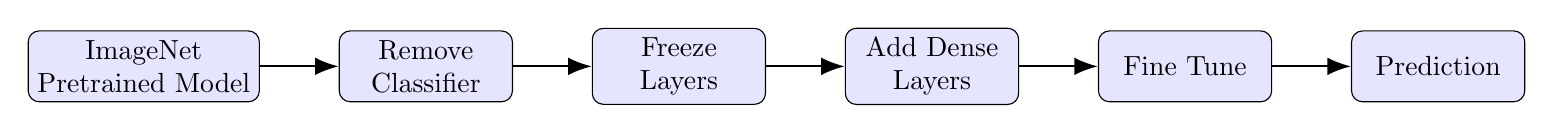
\begin{tikzpicture}[node distance=1cm]

\node[layer](a){ImageNet\\Pretrained Model};
\node[layer,right=of a](b){Remove\\Classifier};
\node[layer,right=of b](c){Freeze\\Layers};
\node[layer,right=of c](d){Add Dense\\Layers};
\node[layer,right=of d](e){Fine Tune};
\node[layer,right=of e](f){Prediction};

\foreach \x/\y in {a/b,b/c,c/d,d/e,e/f}
\draw[arrow](\x)--(\y);

\end{tikzpicture}

\caption{Transfer Learning Workflow}

\end{figure}

Advantages

\begin{itemize}
\item Faster convergence.
\item Higher accuracy on small datasets.
\item Reduced training time.
\item Lower computational cost.
\end{itemize}

%%%%%%%%%%%%%%%%%%%%%%%%%%%%%%%%%%%%%%%%%%%%%%%%%%%%%%%%%%%%

\section*{14. Dataset}

Dataset: CIFAR-10

\begin{itemize}

\item Training Images : 50,000

\item Testing Images : 10,000

\item Number of Classes : 10

\item Image Size : $32\times32\times3$

\item Classes:
Airplane, Automobile, Bird, Cat, Deer,
Dog, Frog, Horse, Ship and Truck.

\end{itemize}

%%%%%%%%%%%%%%%%%%%%%%%%%%%%%%%%%%%%%%%%%%%%%%%%%%%%%%%%%%%%

\section*{15. Experimental Procedure}

\subsection*{Task 1: Dataset Preparation}

\begin{enumerate}

\item Load the CIFAR-10 dataset using TensorFlow/Keras.

\item Normalize the pixel values to the range [0,1].

\item Display ten sample images.

\item Print the dimensions of the training and testing datasets.

\end{enumerate}

%%%%%%%%%%%%%%%%%%%%%%%%%%%%%%%%%%%%%%%%%%%%%%%%%%%%%%%%%%%%

\subsection*{Task 2: Transfer Learning}

Load any one of the following pretrained CNN models.

\begin{itemize}

\item VGG16

\item ResNet50

\item MobileNetV2

\item EfficientNetB0 (Optional)

\end{itemize}

Perform the following steps.

\begin{enumerate}

\item Load pretrained ImageNet weights.

\item Remove the original classification layer.

\item Freeze the convolutional base.

\item Add a Global Average Pooling layer.

\item Add a Dense layer with ReLU activation.

\item Add the output layer with Softmax activation.

\end{enumerate}

%%%%%%%%%%%%%%%%%%%%%%%%%%%%%%%%%%%%%%%%%%%%%%%%%%%%%%%%%%%%

\subsection*{Task 3: Model Training}

Train the model using

\begin{center}

\begin{tabular}{|p{5cm}|p{6cm}|}

\hline

Optimizer & Adam\\

\hline

Learning Rate & 0.001\\

\hline

Batch Size & 32\\

\hline

Epochs & 10--20\\

\hline

Loss Function &
Categorical Cross Entropy\\

\hline

Evaluation Metric &
Accuracy\\

\hline

\end{tabular}

\end{center}

%%%%%%%%%%%%%%%%%%%%%%%%%%%%%%%%%%%%%%%%%%%%%%%%%%%%%%%%%%%%

\subsection*{Task 4: Fine Tuning}

\begin{enumerate}

\item Unfreeze the last convolution block.

\item Train for another 5--10 epochs.

\item Compare the classification accuracy before and after fine tuning.

\end{enumerate}

%%%%%%%%%%%%%%%%%%%%%%%%%%%%%%%%%%%%%%%%%%%%%%%%%%%%%%%%%%%%

\subsection*{Task 5: Model Evaluation}

Evaluate the trained model using

\begin{itemize}

\item Accuracy

\item Precision

\item Recall

\item F1-score

\item Confusion Matrix

\item Classification Report

\end{itemize}

%%%%%%%%%%%%%%%%%%%%%%%%%%%%%%%%%%%%%%%%%%%%%%%%%%%%%%%%%%%%

\section*{16. Hyperparameter Study}

Compare the performance using different settings.

\begin{center}

\begin{tabular}{|l|l|}

\hline

Hyperparameter & Values\\

\hline

Learning Rate &
0.001, 0.0001\\

\hline

Batch Size &
16, 32, 64\\

\hline

Epochs &
10, 20\\

\hline

Optimizer &
Adam, SGD\\

\hline

Dense Units &
128, 256\\

\hline

Frozen Layers &
All, Partial\\

\hline

\end{tabular}

\end{center}

%%%%%%%%%%%%%%%%%%%%%%%%%%%%%%%%%%%%%%%%%%%%%%%%%%%%%%%%%%%%

\section*{17. Mandatory Plots}

Include the following plots in the laboratory report.

\begin{enumerate}

\item Sample CIFAR-10 images

\item Training Accuracy

\item Validation Accuracy

\item Training Loss

\item Validation Loss

\item Confusion Matrix

\item Misclassified Images (Optional)

\end{enumerate}

Students should write a brief inference (2--3 lines) for each figure.

%%%%%%%%%%%%%%%%%%%%%%%%%%%%%%%%%%%%%%%%%%%%%%%%%%%%%%%%%%%%

\section*{18. Results}

\subsection*{18.1 Performance Metrics (VGG16 -- Primary Model)}

\begin{center}
\begin{tabular}{|p{6cm}|p{4cm}|}
\hline
Metric & Value\\
\hline
Training Accuracy                        & 88.49\% \\
\hline
Validation Accuracy (before fine-tuning) & 85.82\% \\
\hline
Validation Accuracy (after fine-tuning)  & 91.14\% \\
\hline
Test Accuracy                            & 91.05\% \\
\hline
Precision                                & 91.61\% \\
\hline
Recall                                   & 91.05\% \\
\hline
F1-score                                 & 91.13\% \\
\hline
Training Time                            & 44.86 min \\
\hline
Fine-Tuning Time                         & 25.81 min \\
\hline
Total Parameters                         & 14,781,642 \\
\hline
\end{tabular}
\end{center}

\vspace{4mm}

\subsection*{18.2 Comparison of CNN Architectures}

\begin{center}
\begin{tabular}{|l|c|c|c|c|c|}
\hline
Model & Parameters & Accuracy (\%) & Precision (\%) & Recall (\%) & Training Time (min)\\
\hline
LeNet-5  & 83,126     & 52.38 & 52.71 & 52.38 & 0.80  \\
\hline
AlexNet  & 36,926,730 & 10.00 &  1.00 & 10.00 & 5.35  \\
\hline
VGG16    & 14,781,642 & \textbf{91.05} & 91.61 & 91.05 & 44.86 \\
\hline
ResNet50 & 23,851,274 & 90.84 & 91.00 & 90.84 & 21.59 \\
\hline
\end{tabular}

\noindent\small\textit{Note: GoogleNet (InceptionV3) was defined in the experimental code but was not executed due to computational constraints. Results are therefore not available.}
\end{center}

\textbf{Summary:} VGG16 achieves the best test accuracy (91.05\%), closely followed by
ResNet50 (90.84\%). LeNet-5 reaches only 52.38\% because its shallow architecture was
designed for small greyscale images, not CIFAR-10 RGB. AlexNet stagnates at 10\%
(random-chance baseline) due to architectural incompatibility with upscaled CIFAR-10.

%%%%%%%%%%%%%%%%%%%%%%%%%%%%%%%%%%%%%%%%%%%%%%%%%%%%%%%%%%%%
\section*{19. Plots and Inferences}

\subsection*{19.1 Plot 1: CIFAR-10 Class Distribution}

\begin{figure}[H]
\centering
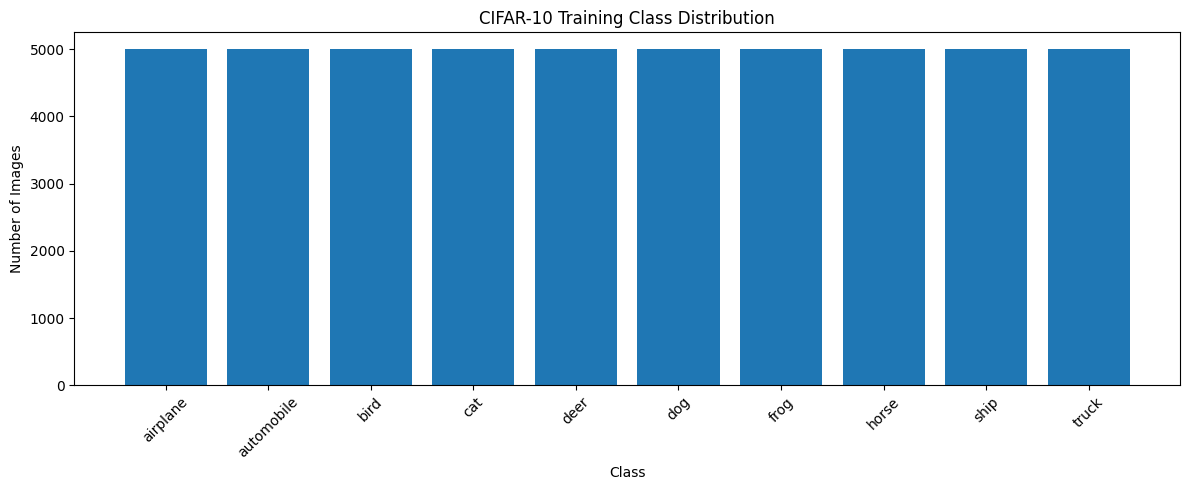
\includegraphics[width=0.85\textwidth]{plots/cell_11_out_0.png}
\caption{CIFAR-10 Training Set -- Class Distribution}
\label{fig:class_dist}
\end{figure}

\textbf{Inference:}
The CIFAR-10 training set is perfectly balanced, with each of the 10 classes containing
exactly 5,000 samples. This balance ensures that the model is not biased towards any
particular class and accuracy can be used directly as the primary evaluation metric
without correction for class imbalance.

\subsection*{19.2 Plot 2: Sample CIFAR-10 Images}

\begin{figure}[H]
\centering
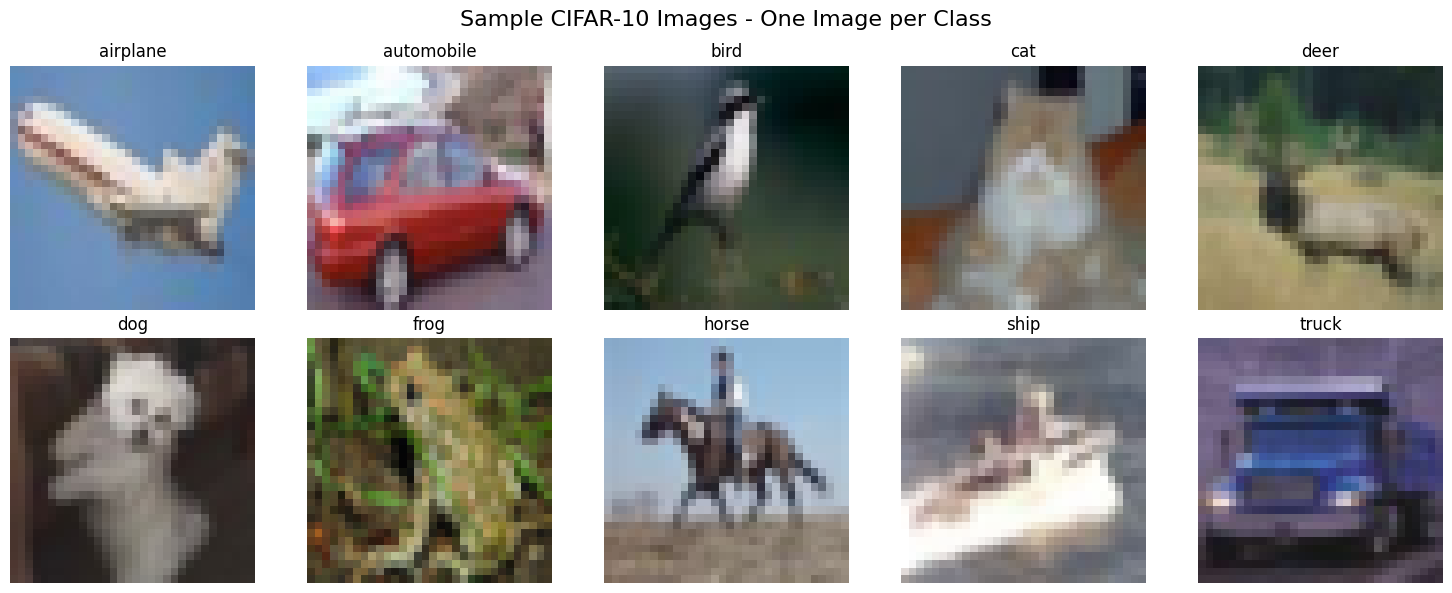
\includegraphics[width=0.90\textwidth]{plots/cell_12_out_0.png}
\caption{One Sample Image from Each CIFAR-10 Class}
\label{fig:sample_images}
\end{figure}

\textbf{Inference:}
The sample images illustrate the diversity and challenge of the CIFAR-10 dataset. The
low resolution ($32\times32$ pixels) and high inter-class visual similarity (e.g., cat
vs.\ dog, automobile vs.\ truck) make this a non-trivial classification task. Transfer
learning from ImageNet-pretrained weights provides a significant advantage by leveraging
rich, generalised feature representations learned from millions of high-resolution images.

\subsection*{19.3 Plot 3: Training and Validation Accuracy (VGG16)}

\begin{figure}[H]
\centering
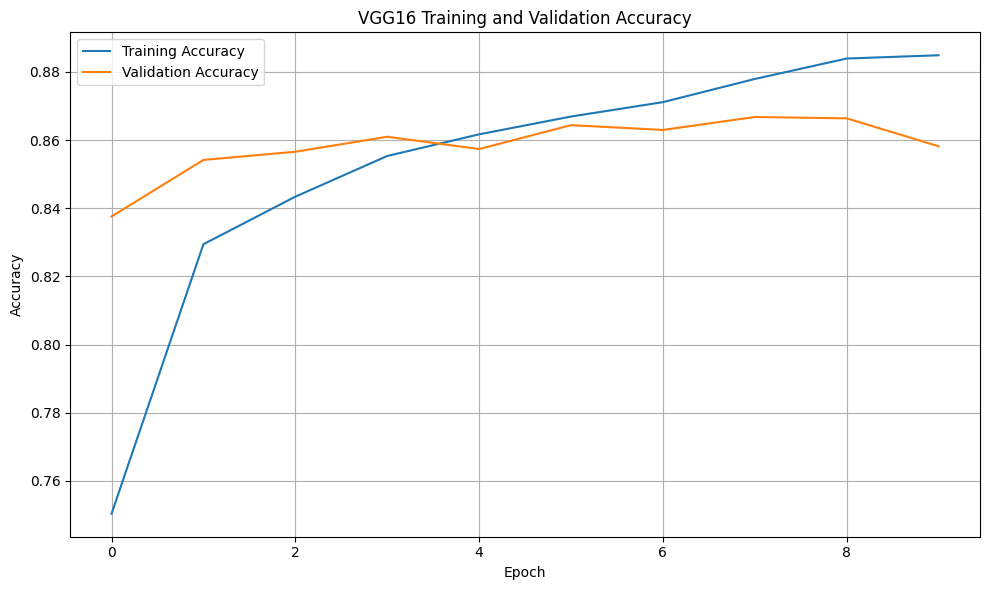
\includegraphics[width=0.85\textwidth]{plots/cell_22_out_0.png}
\caption{VGG16 Training and Validation Accuracy versus Epoch}
\label{fig:vgg_acc}
\end{figure}

\textbf{Inference:}
Training accuracy rises steadily from approximately 75\% to 88.5\% over 10 epochs,
while validation accuracy closely follows, reaching 85.8\%. The small train--val gap
($\approx$2.7\%) indicates good generalisation without significant overfitting, which is
expected since the convolutional base is frozen and only the newly added classification
head is being trained.

\subsection*{19.4 Plot 4: Training and Validation Loss (VGG16)}

\begin{figure}[H]
\centering
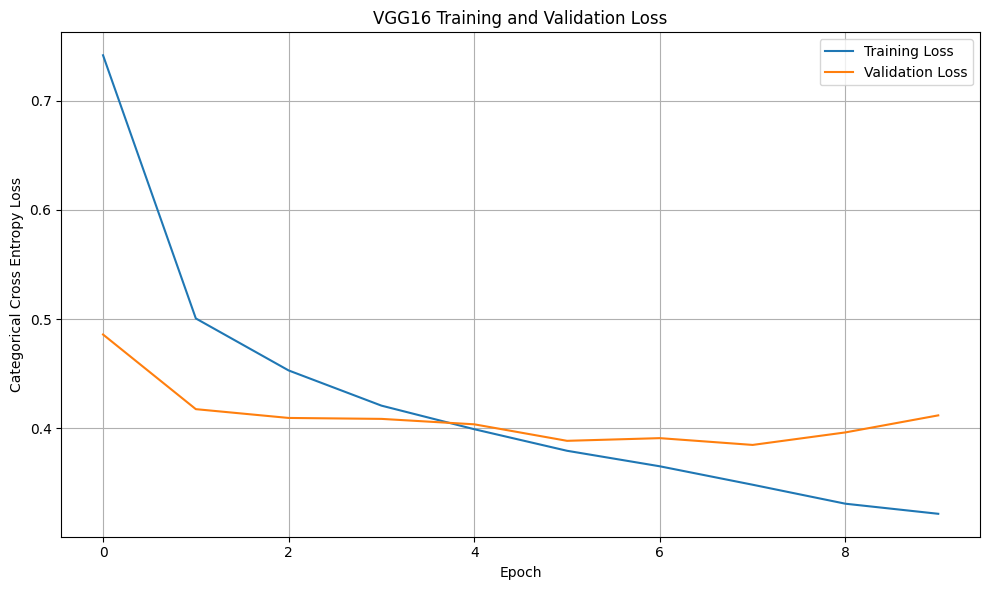
\includegraphics[width=0.85\textwidth]{plots/cell_23_out_0.png}
\caption{VGG16 Training and Validation Loss versus Epoch}
\label{fig:vgg_loss}
\end{figure}

\textbf{Inference:}
Both training and validation losses decrease smoothly across all 10 epochs, confirming
stable optimisation with Adam (lr = 0.001). The two loss curves remain closely aligned,
showing no divergence that would indicate overfitting. The monotone decrease also
confirms that the learning rate is well chosen for fine-tuning the classification head.

\subsection*{19.5 Plot 5: Before vs After Fine-Tuning (VGG16)}

\begin{figure}[H]
\centering
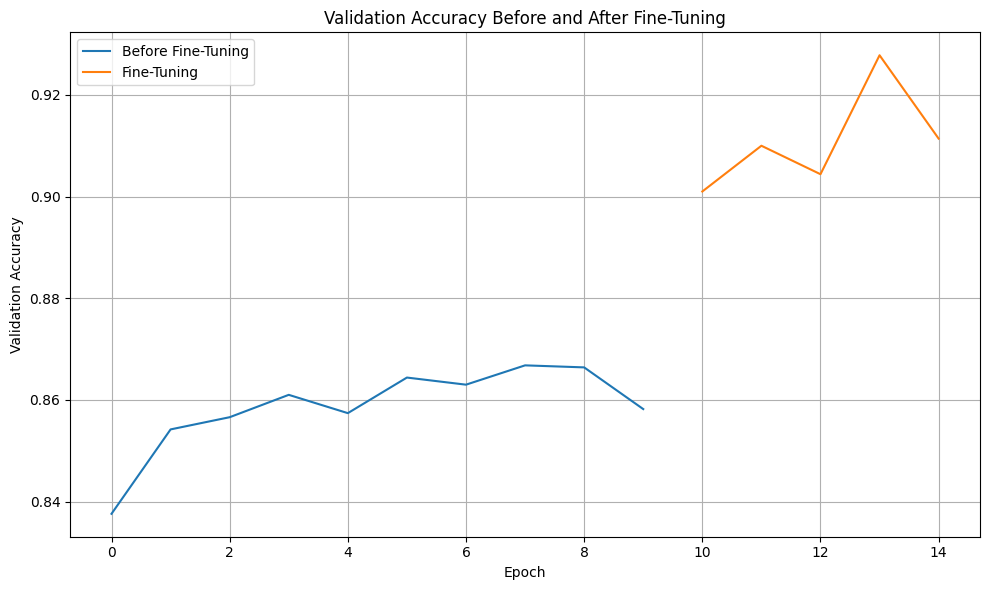
\includegraphics[width=0.85\textwidth]{plots/cell_28_out_0.png}
\caption{VGG16 Validation Accuracy: Feature Extraction vs.\ Fine-Tuning}
\label{fig:finetune}
\end{figure}

\textbf{Inference:}
Fine-tuning the last convolutional block improves the best validation accuracy from
85.82\% to 91.14\%, a gain of 5.3 percentage points. This demonstrates that higher-level
VGG16 features, though pretrained on ImageNet, can be meaningfully adapted to the
CIFAR-10 domain. The gain justifies the additional 25.8 minutes of fine-tuning
computation.

\subsection*{19.6 Plot 6: Confusion Matrix (VGG16)}

\begin{figure}[H]
\centering
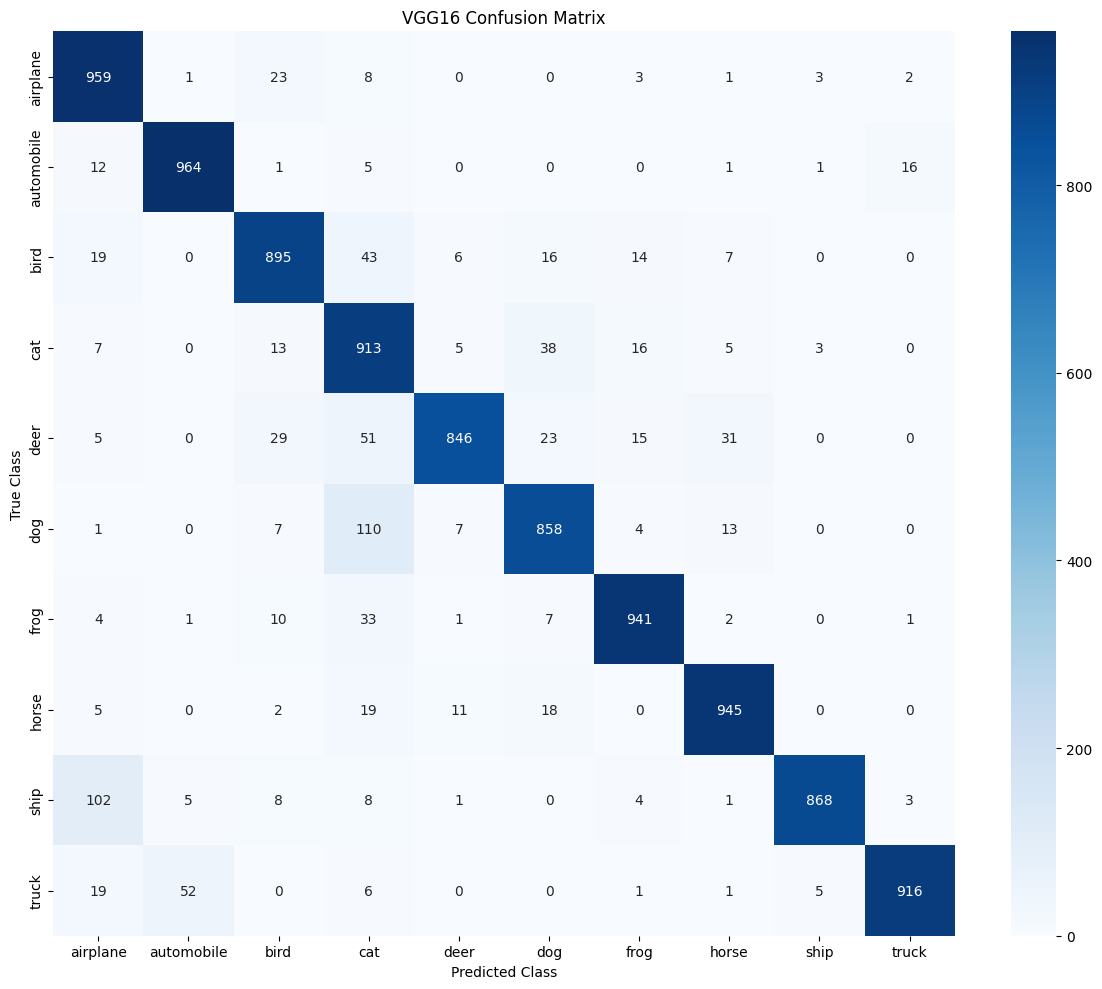
\includegraphics[width=0.90\textwidth]{plots/cell_33_out_0.png}
\caption{Confusion Matrix on the CIFAR-10 Test Set (VGG16 after Fine-Tuning)}
\label{fig:confusion}
\end{figure}

\textbf{Inference:}
The confusion matrix shows strong diagonal dominance, indicating consistently high
per-class accuracy. The most frequent confusions occur between visually similar classes:
cat $\leftrightarrow$ dog and automobile $\leftrightarrow$ truck. These errors are
expected at $32\times32$ resolution. Classes such as automobile and ship achieve
$>$96\% accuracy owing to their distinctive visual features.

\subsection*{19.7 Plot 7: Per-Class Test Accuracy (VGG16)}

\begin{figure}[H]
\centering
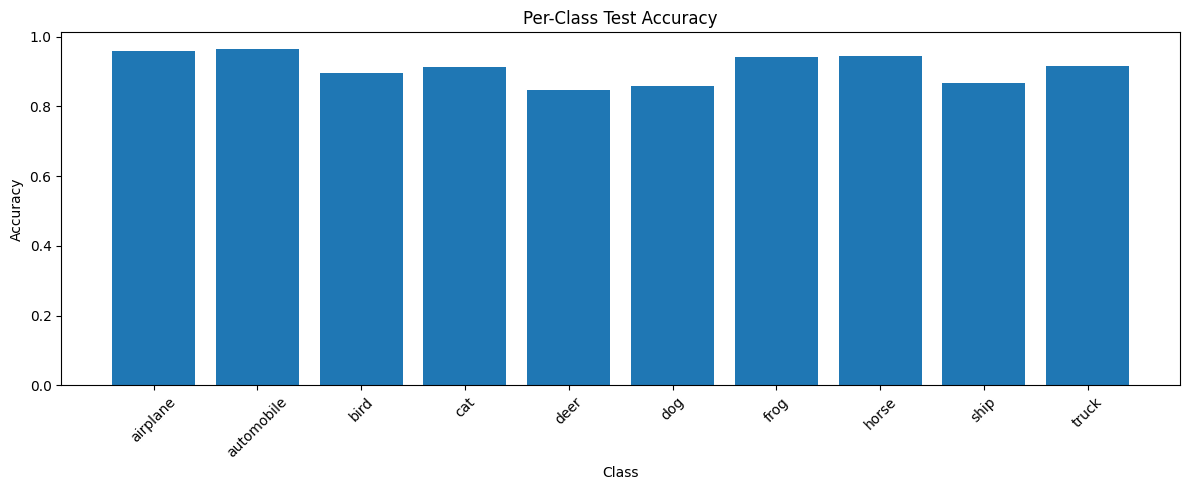
\includegraphics[width=0.85\textwidth]{plots/cell_35_out_0.png}
\caption{Per-Class Test Accuracy for VGG16 on CIFAR-10}
\label{fig:perclass}
\end{figure}

\textbf{Inference:}
Automobile (96.4\%) and airplane (95.9\%) achieve the highest per-class accuracy, while
deer (84.6\%) and dog (85.8\%) are weakest. The lower performance on cat and deer stems
from their visual overlap with dog and horse respectively. The overall accuracy of
91.05\% reflects a well-performing model with no catastrophically weak class.

\subsection*{19.8 Plot 8: Misclassified Images (VGG16)}

\begin{figure}[H]
\centering
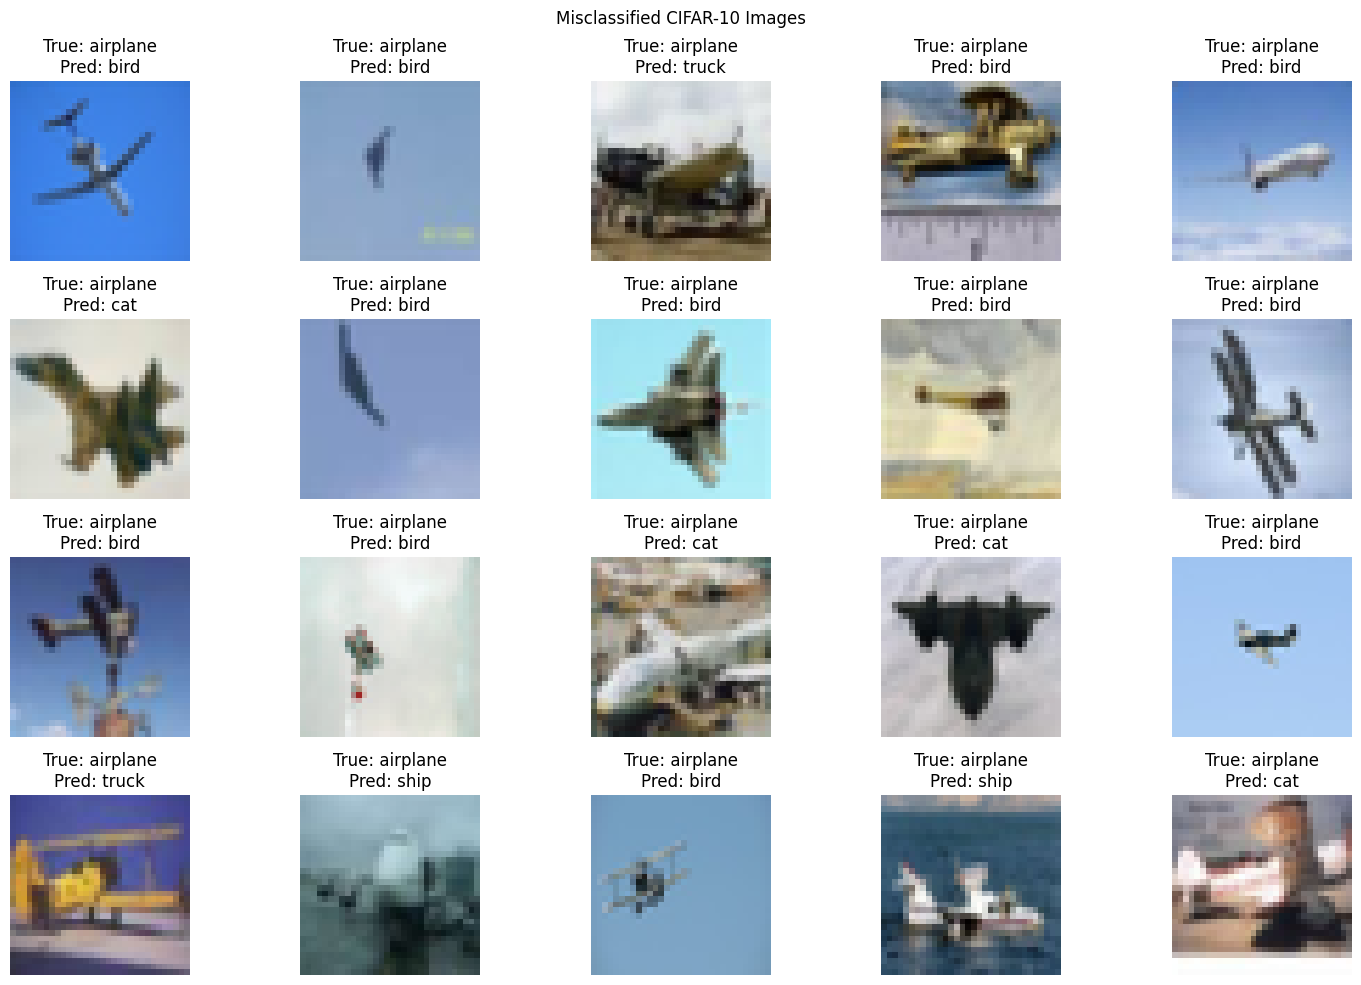
\includegraphics[width=0.90\textwidth]{plots/cell_36_out_0.png}
\caption{Representative Misclassified Images from the Test Set}
\label{fig:misclassified}
\end{figure}

\textbf{Inference:}
Of the 10,000 test images, 895 (8.95\%) are misclassified. The errors predominantly
arise from challenging viewpoints, partial occlusion, and high inter-class similarity.
Many misclassified samples are genuinely ambiguous even to a human observer, suggesting
that the remaining error is close to the irreducible Bayes error for CIFAR-10 at
$32\times32$ resolution.

\subsection*{19.9 Plot 9: Architecture Accuracy Comparison}

\begin{figure}[H]
\centering
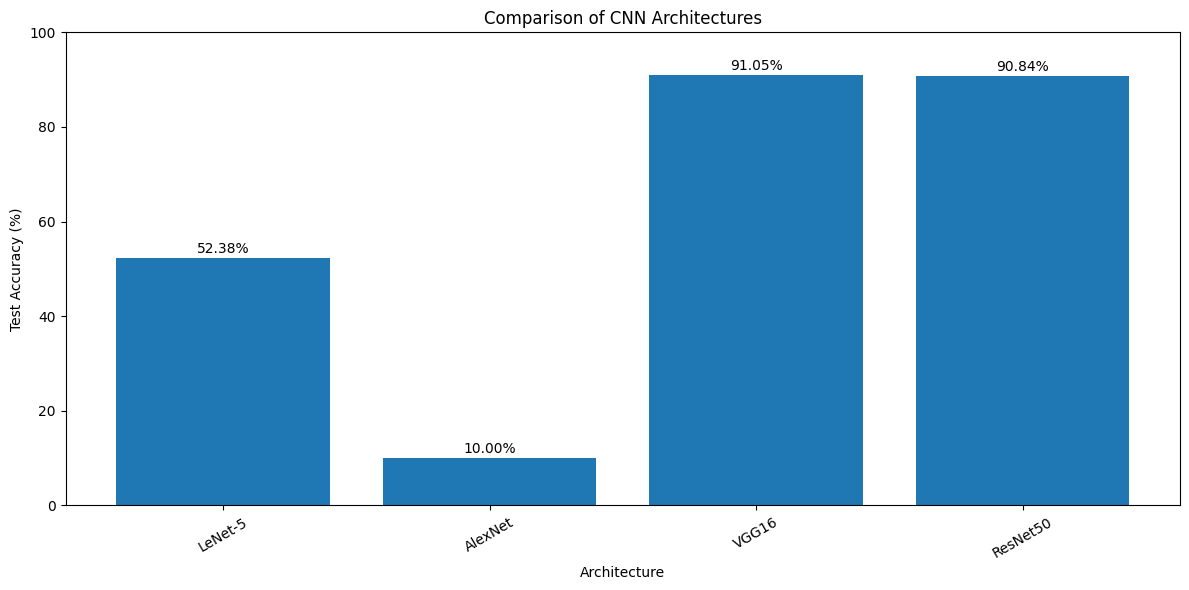
\includegraphics[width=0.85\textwidth]{plots/cell_55_out_0.png}
\caption{Test Accuracy Comparison Across CNN Architectures}
\label{fig:arch_acc}
\end{figure}

\textbf{Inference:}
VGG16 achieves the best test accuracy (91.05\%), closely followed by ResNet50 (90.84\%).
LeNet-5 reaches only 52.38\% -- expected since its shallow 7-layer architecture cannot
capture the complex features in CIFAR-10. AlexNet stagnates at 10\% (random chance),
because its architecture is ill-suited for CIFAR-10 without significant input
adaptation.

\subsection*{19.10 Plot 10: Training Time Comparison}

\begin{figure}[H]
\centering
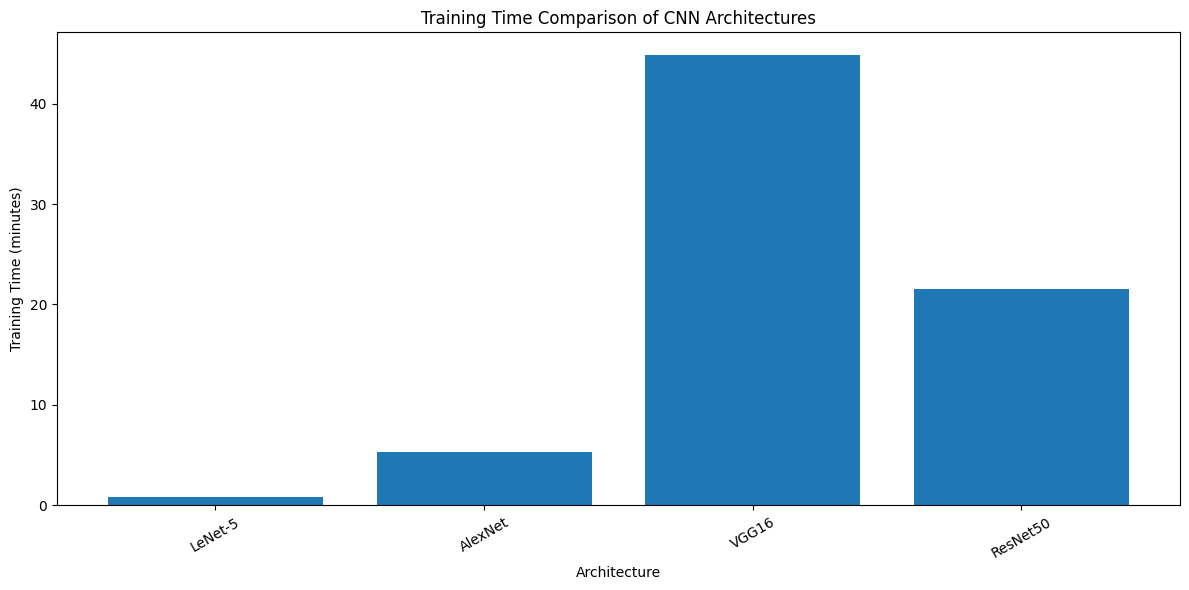
\includegraphics[width=0.85\textwidth]{plots/cell_58_out_0.png}
\caption{Training Time (minutes) Comparison Across CNN Architectures}
\label{fig:arch_time}
\end{figure}

\textbf{Inference:}
VGG16 requires the longest training time (44.86 min) owing to its deep architecture,
even with the convolutional base frozen. ResNet50 trains in 21.59 min despite having
50 layers, because residual connections enable faster gradient propagation. LeNet-5 is
the fastest (0.80 min) due to its minimal depth and parameter count, illustrating the
classic accuracy--efficiency trade-off.

\subsection*{19.11 Plot 11: Parameter Count Comparison}

\begin{figure}[H]
\centering
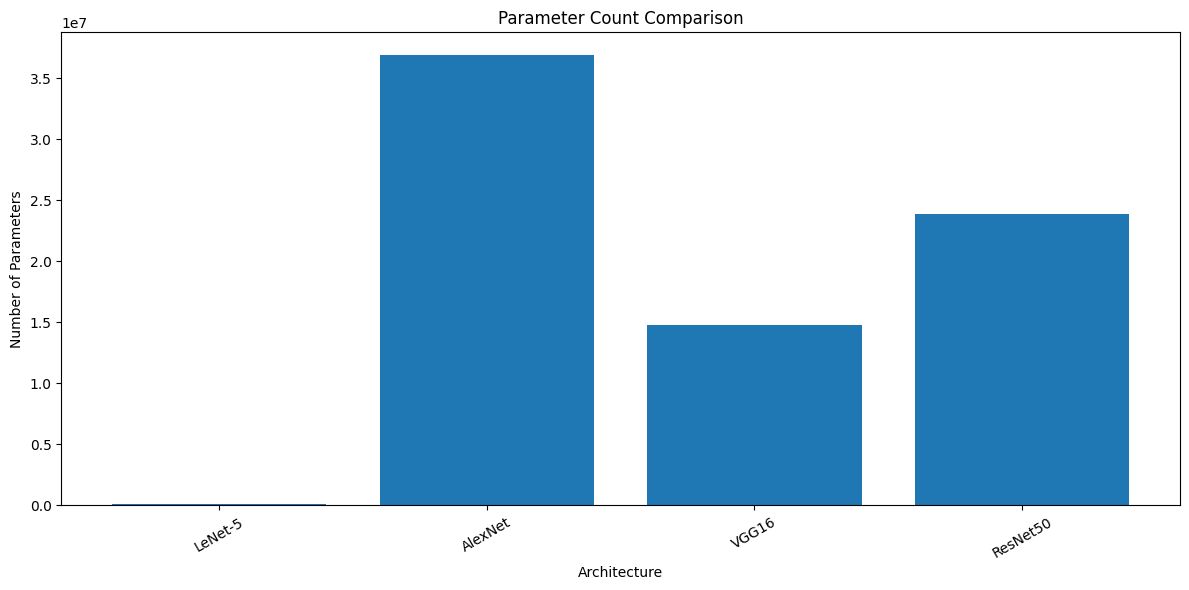
\includegraphics[width=0.85\textwidth]{plots/cell_59_out_0.png}
\caption{Number of Parameters Comparison Across CNN Architectures}
\label{fig:arch_params}
\end{figure}

\textbf{Inference:}
AlexNet has the most parameters (36.9M) yet delivers the worst accuracy, confirming
that parameter count alone does not determine performance. ResNet50 achieves near-VGG16
accuracy with 23.8M parameters, demonstrating the efficiency of residual learning.
LeNet-5's 83K parameters are sufficient only within its intended domain.

\subsection*{19.12 Plot 12: Combined Architecture Comparison}

\begin{figure}[H]
\centering
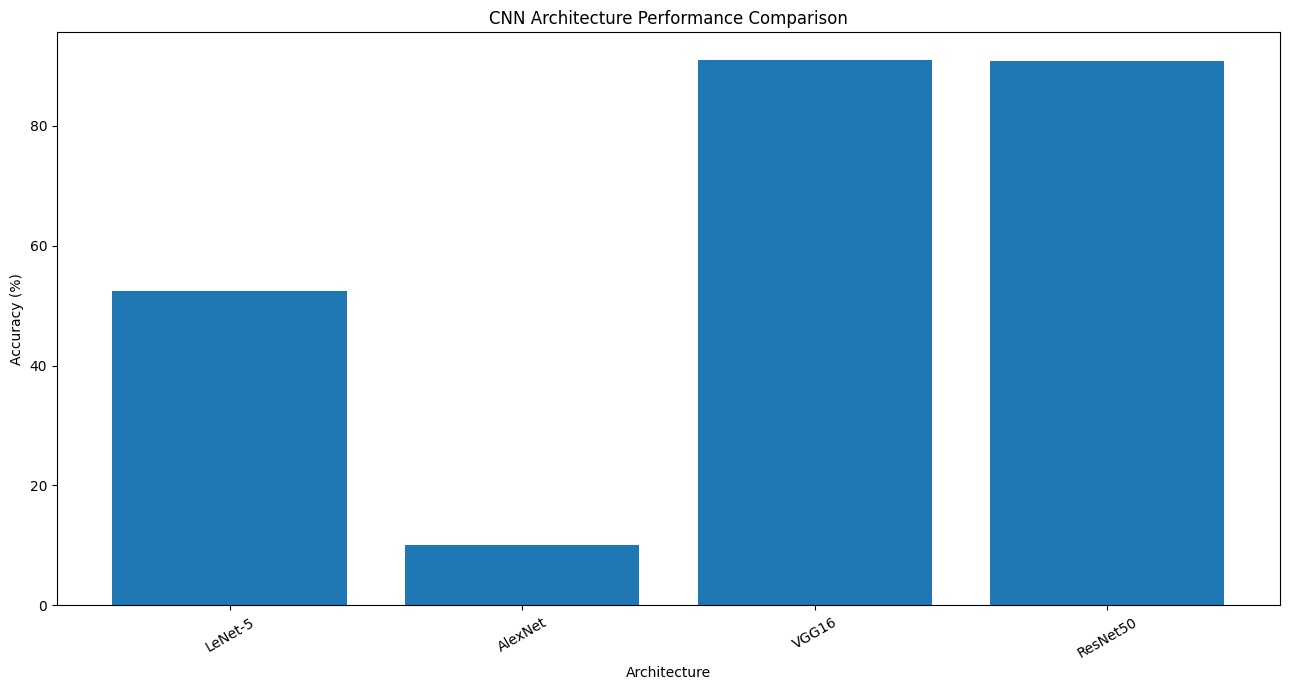
\includegraphics[width=0.95\textwidth]{plots/cell_62_out_0.png}
\caption{Combined Comparison: Accuracy, Parameters and Training Time}
\label{fig:combined}
\end{figure}

\textbf{Inference:}
This combined chart reveals that VGG16 and ResNet50 occupy a similar accuracy tier
($\approx$91\%), but ResNet50 achieves this with fewer parameters and shorter training
time, making it more efficient in resource-constrained environments. AlexNet is the
worst performer across all three dimensions simultaneously, confirming it is unsuitable
for CIFAR-10 without significant architectural adaptation.

%%%%%%%%%%%%%%%%%%%%%%%%%%%%%%%%%%%%%%%%%%%%%%%%%%%%%%%%%%%%

\section*{20. Discussion Questions}

Answer the following questions.

\begin{enumerate}

\item Why is AlexNet considered a breakthrough in deep learning?

\item Why does VGG16 use only $3\times3$ convolution filters?

\item Explain the advantages of the Inception module.

\item What is the purpose of residual learning?

\item Differentiate LeNet and ResNet.

\item What is Transfer Learning?

\item Why is fine tuning required?

\item Explain the difference between dilated convolution and transpose convolution.

\item Why do pretrained models converge faster?

\item Compare the computational complexity of LeNet and ResNet.

\end{enumerate}

%%%%%%%%%%%%%%%%%%%%%%%%%%%%%%%%%%%%%%%%%%%%%%%%%%%%%%%%%%%%

\section*{21. Additional Exercises}

\begin{enumerate}

\item Implement transfer learning using VGG16.

\item Repeat the experiment using ResNet50.

\item Compare Adam and SGD optimizers.

\item Compare training with frozen layers and fine tuning.

\item Evaluate the model using Precision, Recall and F1-score.

\item Compare the performance of LeNet, AlexNet and ResNet.

\end{enumerate}

%%%%%%%%%%%%%%%%%%%%%%%%%%%%%%%%%%%%%%%%%%%%%%%%%%%%%%%%%%%%

\section*{22. References}

\begin{enumerate}

\item Yann LeCun, Leon Bottou, Yoshua Bengio and Patrick Haffner,
\emph{Gradient-Based Learning Applied to Document Recognition},
Proceedings of the IEEE, 1998.

\item Alex Krizhevsky, Ilya Sutskever and Geoffrey Hinton,
\emph{ImageNet Classification with Deep Convolutional Neural Networks},
NeurIPS, 2012.

\item Karen Simonyan and Andrew Zisserman,
\emph{Very Deep Convolutional Networks for Large-Scale Image Recognition},
ICLR, 2015.

\item Christian Szegedy et al.,
\emph{Going Deeper with Convolutions},
CVPR, 2015.

\item Kaiming He, Xiangyu Zhang, Shaoqing Ren and Jian Sun,
\emph{Deep Residual Learning for Image Recognition},
CVPR, 2016.

\item Ian Goodfellow, Yoshua Bengio and Aaron Courville,
\emph{Deep Learning},
MIT Press, 2016.

\item TensorFlow Documentation:
\url{https://www.tensorflow.org}

\item Keras Documentation:
\url{https://keras.io}

\end{enumerate}

%%%%%%%%%%%%%%%%%%%%%%%%%%%%%%%%%%%%%%%%%%%%%%%%%%%%%%%%%%%%

\end{document}
